%===============================================================================
% LaTeX sjabloon voor de bachelorproef toegepaste informatica aan HOGENT
% Meer info op https://github.com/HoGentTIN/latex-hogent-report
%===============================================================================

\documentclass[dit,thesis]{hogentreport}

% TODO:
% - If necessary, replace the option `dit`' with your own department!
%   Valid entries are dbo, dbt, dgz, dit, dlo, dog, dsa, soa
% - If you write your thesis in English (remark: only possible after getting
%   explicit approval!), remove the option "dutch," or replace with "english".

\usepackage{lipsum} % For blind text, can be removed after adding actual content

%% Pictures to include in the text can be put in the graphics/ folder
\graphicspath{{../graphics/}}

%% For source code highlighting, requires pygments to be installed
%% Compile with the -shell-escape flag!
%% \usepackage[chapter]{minted}
%% If you compile with the make_thesis.{bat,sh} script, use the following
%% import instead:
\usepackage[chapter,outputdir=../output]{minted}
\usemintedstyle{solarized-light}

%% Formatting for minted environments.
\setminted{%
    autogobble,
    frame=lines,
    breaklines,
    linenos,
    tabsize=4
}

%% Ensure the list of listings is in the table of contents
\renewcommand\listoflistingscaption{%
    \IfLanguageName{dutch}{Lijst van codefragmenten}{List of listings}
}
\renewcommand\listingscaption{%
    \IfLanguageName{dutch}{Codefragment}{Listing}
}
\renewcommand*\listoflistings{%
    \cleardoublepage\phantomsection\addcontentsline{toc}{chapter}{\listoflistingscaption}%
    \listof{listing}{\listoflistingscaption}%
}

% Other packages not already included can be imported here

%%---------- Document metadata -------------------------------------------------
% TODO: Replace this with your own information
\author{Ernst Aarden}
\supervisor{Dhr. F. Van Houte}
\cosupervisor{Mevr. S. Beeckman}
\title[Optionele ondertitel]%
    {Titel van de bachelorproef}
\academicyear{\advance\year by -1 \the\year--\advance\year by 1 \the\year}
\examperiod{1}
\degreesought{\IfLanguageName{dutch}{Professionele bachelor in de toegepaste informatica}{Bachelor of applied computer science}}
\partialthesis{false} %% To display 'in partial fulfilment'
%\institution{Internshipcompany BVBA.}

%% Add global exceptions to the hyphenation here
\hyphenation{back-slash}

%% The bibliography (style and settings are  found in hogentthesis.cls)
\addbibresource{bachproef.bib}            %% Bibliography file
\addbibresource{../voorstel/voorstel.bib} %% Bibliography research proposal
\defbibheading{bibempty}{}

%% Prevent empty pages for right-handed chapter starts in twoside mode
\renewcommand{\cleardoublepage}{\clearpage}

\renewcommand{\arraystretch}{1.2}

%% Content starts here.
\begin{document}

%---------- Front matter -------------------------------------------------------

\frontmatter

\hypersetup{pageanchor=false} %% Disable page numbering references
%% Render a Dutch outer title page if the main language is English
\IfLanguageName{english}{%
    %% If necessary, information can be changed here
    \degreesought{Professionele Bachelor toegepaste informatica}%
    \begin{otherlanguage}{dutch}%
       \maketitle%
    \end{otherlanguage}%
}{}

%% Generates title page content
\maketitle
\hypersetup{pageanchor=true}

\input{voorwoord}
\input{samenvatting}

%---------- Inhoud, lijst figuren, ... -----------------------------------------

\tableofcontents

% In a list of figures, the complete caption will be included. To prevent this,
% ALWAYS add a short description in the caption!
%
%  \caption[short description]{elaborate description}
%
% If you do, only the short description will be used in the list of figures

\listoffigures

% If you included tables and/or source code listings, uncomment the appropriate
% lines.
\listoftables

\listoflistings

% Als je een lijst van afkortingen of termen wil toevoegen, dan hoort die
% hier thuis. Gebruik bijvoorbeeld de ``glossaries'' package.
% https://www.overleaf.com/learn/latex/Glossaries

%---------- Kern ---------------------------------------------------------------

\mainmatter{}

% De eerste hoofdstukken van een bachelorproef zijn meestal een inleiding op
% het onderwerp, literatuurstudie en verantwoording methodologie.
% Aarzel niet om een meer beschrijvende titel aan deze hoofdstukken te geven of
% om bijvoorbeeld de inleiding en/of stand van zaken over meerdere hoofdstukken
% te verspreiden!

\input{inleiding}
\input{standvanzaken}
\input{methodologie}

% Voeg hier je eigen hoofdstukken toe die de ``corpus'' van je bachelorproef
% vormen. De structuur en titels hangen af van je eigen onderzoek. Je kan bv.
% elke fase in je onderzoek in een apart hoofdstuk bespreken.

%\input{...}
%\input{...}
%...

\input{conclusie}

%---------- Bijlagen -----------------------------------------------------------

\appendix

\chapter{Onderzoeksvoorstel}

Het onderwerp van deze bachelorproef is gebaseerd op een onderzoeksvoorstel dat vooraf werd beoordeeld door de promotor. Dat voorstel is opgenomen in deze bijlage.

%% TODO: 
%\section*{Samenvatting}

% Kopieer en plak hier de samenvatting (abstract) van je onderzoeksvoorstel.

% Verwijzing naar het bestand met de inhoud van het onderzoeksvoorstel
%---------- Inleiding ---------------------------------------------------------

% TODO: Is dit voorstel gebaseerd op een paper van Research Methods die je
% vorig jaar hebt ingediend? Heb je daarbij eventueel samengewerkt met een
% andere student?
% Zo ja, haal dan de tekst hieronder uit commentaar en pas aan.

%\paragraph{Opmerking}

% Dit voorstel is gebaseerd op het onderzoeksvoorstel dat werd geschreven in het
% kader van het vak Research Methods dat ik (vorig/dit) academiejaar heb
% uitgewerkt (met medesturent VOORNAAM NAAM als mede-auteur).
% 

\section{Introduction}%
\label{sec:Introduction}
Quality assurance plays an indispensable role in everyday software development. In environments where continuous new improvements are implemented, we cannot afford to waste time, which unfortunately often happens during the final step of integrating new code. Therefore, detecting errors in software promptly is crucial to preventing issues during and after release.
With this research, we aim to address a specific issue faced by Wolters Kluwer: resolving errors in new code integrations. As technology has evolved, we have moved from manual to automated testing, with visual testing proven as an effective approach. The next step is obviously to use AI to speed up the resolution of errors. 
In this bachelor’s thesis, we investigate how AI can be used to improve the automated process of visual testing within CI/CD pipelines. Our focus is primarily on reducing the debugging time required after a test fails, using AI. Through a proof-of-concept, we aim to demonstrate how AI can detect visual errors and identify the associated code.
Furthermore, we will experiment with how AI can implement self-healing; in other words, how AI can devise its solution to a problem that arises. Our focus is specifically on exploring how AI can optimize the debugging process, with the goal of minimizing both time and the need for manual intervention.

%---------- Stand van zaken ---------------------------------------------------

\section{State-of-the-art}%
\label{sec:State-of-the-art}
When CI/CD is implemented, code quality is improved, and software updates are delivered rapidly with high confidence that they won't introduce breaking modifications.
Automated testing has become an indispensable component of successful CI/CD pipelines and is key to ensuring quality and reliability.
By reducing the amount of manual effort necessary, we can accelerate the delivery of high-quality software.
One of the ways to do this is by utilizing AI techniques for multiple components of automated testing.
Topics such as test case generation, test prioritization, defect prediction, and self-healing tests are promising techniques that, while not yet fully developed or researched, hold great potential for the future and their adaptation in CI/CD pipelines will bring great value. 
\autocite{Kaniganti}
Self-healing tests are a proven concept and are services offered by multiple test frameworks. The main objective is to fix simple problems that are time-consuming. The AI is dynamic and can handle problems while not requiring human attention or manual labor.\autocite{Shabarish2024}
AI-driven test automation is now face-changing software testing, ranging from functional, performance, and visual testing by off-loading much of these tasks from human testers. For instance, techniques of automated visual testing use AI in performing the detection of visual appearances of GUI bugs that might be left unnoticed by other testing methods. These tools can analyze screenshots, perform object detection, and classify changes to improve the quality of user interfaces.
\autocite{Gamal2023}
AI applications in automated testing have various methodologies associated with them. In some cases, for example, visual GUI testing employs image recognition to simulate human activities; hence, it allows more dynamic interfaces to be tested.
\autocite{BaniMuhamad2016}
Along with this, AI-enabled techniques like machine learning and computer vision applied to the testing tool help make the tests more dynamic with software changes and generate and execute better test cases.
\autocite{Trudova.2020}
AI debugging tools parse lines of code, finding potential issues faster and more effectively than any human manual method could. Generative AI creates new test cases and data to find those bugs hidden deep inside complex systems, such as neural networks.
\autocite{Staron2024}
This facility speeds up the debugging process and decreases manual effort, thus saving the developers for more critical work.
AI plays a major role in amplifying CI/CD practices with the automation of integration and deployment. AI-driven CI/CD tools can track changes to code, automatically perform tests, and carry out application deployment with as little human interference as possible, ultimately attaining quicker speeds while not compromising on reliability in software delivery.
\autocite{Mohammed2024}
This automation supports high-quality standards with rapid changes in software requirements.
On the other hand, the advantages have their own challenges. For example, there is an immense requirement for robust training data in AI integration within software engineering. Then again, there might be error introductions because of the complete reliance on AI algorithms. With increasing research, the field is trying to evolve more enhanced models and tools of AI which can handle such complexities of testing and debugging software.
\autocite{Steidl2023}
Traditional visual testing relies on pixel-by-pixel comparisons, which results in a number of false positives due to minor rendering differences, like anti-aliasing effects. AI can include context-aware analysis: it understands the meaning of spatial relationships and the contextual significance of every UI element. AI would, for example, distinguish between acceptable variations-like slight color changes based on display settings-and actual defects.
\autocite{Moradi2024}
% Voor literatuurverwijzingen zijn er twee belangrijke commando's:
% \autocite{KEY} => (Auteur, jaartal) Gebruik dit als de naam van de auteur
%   geen onderdeel is van de zin.
% \textcite{KEY} => Auteur (jaartal)  Gebruik dit als de auteursnaam wel een
%   functie heeft in de zin (bv. ``Uit onderzoek door Doll & Hill (1954) bleek
%   ...'')

%---------- Methodologie ------------------------------------------------------
\section{Methodology}%
\label{sec:methodology}
In the first phase, the objective is to gather sophisticated knowledge about the subject.
The purpose is to gather and deconstruct academic papers, relevant articles, and manuals that articulate the concepts of debugging and automated testing.
Furthermore, this research will concentrate on examining contemporary technologies that contribute to advancements in debugging practices, alongside an examination of the current usages of artificial intelligence in optimizing debugging processes.
The techniques we find to be currently used will be examined and and researched.
Ending the first phase, we will set clear objectives and criteria to determine the future of this research.
The different use cases of AI will be compared to each other and a determination will be made of which of these use cases is most fit and feasable to produce.
In the third phase a determination will be made of which AI tool will be used and if there are any frameworks or technologies that already made advancements useful for this study.
Following the third phase will be used to gather the correct application(s) and data to test and make a proof-of-concept around.
It's very important that this application has a broad scala of functions and data to be tested.
In the fifth phase the proof-of-concept will be fabricated on a specific technique of how AI can help debugging in a visual testing scenario.
Which resources are required will be dependent on which solution we will work on, determined in phase 2.
The model will be trained with the data we gathered in the third phase.
After the proof-of-concept is finished, the possibilities to implement this inside of a CI/CD pipeline will be researched.
A recommendation will be written on how to implement the most workable and efficiënt model to use inside of an automated testing environment.
\begin{figure}[h]
    \centering
    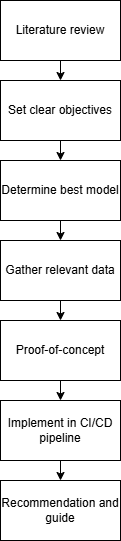
\includegraphics[scale=0.4]{../graphics/BPVOORSTELVITODEDECKER.drawio.png}
    \caption{VisualRepresentation}
    \label{fig:VisualRepresentation}
\end{figure}
%---------- Verwachte resultaten ----------------------------------------------
\section{Expected results}%
\label{sec:Expected results}

By studying the available AI-powered debugging and visual testing solutions, we should be in a position to ascertain whether the effort of developing a similar solution would be expedient or not for integration into a CI/CD pipeline. Given the unrelenting demand for efficiency in error resolution and the rarity of widely embraced AI-powered solutions in the realm of visual testing, there is certainly every reason to believe that an implementation of a custom AI solution will carry significant value with it.
This proof of concept can help reduce error detection, debugging time, and manual efforts being invested in software quality by providing quick and reliable ways of software release. There is little or no competition in this AI-assisted visual debugging solution in the continuous integration/continuous deployment segment, and the market opportunity looks good for the solution.



%%---------- Andere bijlagen --------------------------------------------------
% TODO: Voeg hier eventuele andere bijlagen toe. Bv. als je deze BP voor de
% tweede keer indient, een overzicht van de verbeteringen t.o.v. het origineel.
%\input{...}

%%---------- Backmatter, referentielijst ---------------------------------------

\backmatter{}

\setlength\bibitemsep{2pt} %% Add Some space between the bibliograpy entries
\printbibliography[heading=bibintoc]

\end{document}
